\documentclass[letterpaper]{article}
\usepackage[top=1.0in,bottom=1.0in,left=1.0in,right=1.0in]{geometry}
\usepackage{verbatim}
\usepackage{amssymb}
\usepackage{graphicx}
\usepackage{svg}
\usepackage{longtable}
\usepackage{amsfonts}
\usepackage{amsmath}
\usepackage{hyperref}
\usepackage{float}
\usepackage{caption}
\usepackage{xcolor}
\usepackage{makecell}
\def\thesection       {\arabic{section}}
\def\thesubsection     {\thesection.\alph{subsection}}

\author{Zoe Richter
        \\ \href{mailto:zrichte2@illinois.edu}{\texttt{zrichte2@illinois.edu}}
}

\title{Reactor Design Compilation}
\begin{document}
%\clearpage
\begin{titlepage}
\maketitle
\thispagestyle{empty}
\end{titlepage}

\section{Introduction}
Molten salt reactors, or MSRs, are a hopeful candidate for the next line of commerical nuclear reactors.  However, there is a lack of experiental data and real-world experience compared to the light-water reactors that make up much of the world's current fleet.

This report seeks to collect various MSR designs and reprocessing techniques, provide an idea of the range of MSR features.  The intent is to capture the expected varieties of fluid-fueled MSRs such that models and simulations can accommodate a broad range of designs.  The features given in this review include characteristics such as:

\begin{itemize}
\item Single fluid or two fluid salt
\item Single or multi-region core
\item Neutron energy spectrum
\item Moderator type
\item Salt type (relates to single or two-fluid)
\item Intensity of processing
\end{itemize}

The processing methods for each reactor will also be given, in as much detail as possible.  The goal is to collect information of possible MSR processing methods in one place, and, to give a better idea of the general trends in fuel-processing methodologies.

To begin, take note of \cite{macpherson_molten_1985} and \cite{rosenthal_molten-salt_1970}.  These articles are not specific designs, instead, they give a general history of US MSR technology up to approximately 1980. \emph{The Molten Salt Adventure}, \cite{macpherson_molten_1985}, in particular, is a personal account of the author's experience in the growing field, and offers interesting insight.\\

\section{Molten Salt Reactor Experiment (MSRE)}
This reactor is given as the first MSR design.  Technically, the Aircraft Reactor Experiment is its predecessor, however, given its unsuitability as a commercial reactor (and the focus of this report on such reactors) it is not included in detail here.  The MSRE has general characteristics, described thusly: \cite{robertson_msre_1965}

\begin{center}
\begin{tabular}{|c|c|}
\hline
MWth & 10\\
\hline
MWe & Not Given \\
\hline
Spectrum & Thermal \\
\hline
Core Inlet Temperature & 635 C \\
\hline
Core Outlet Temperature & 663 C\\
\hline
Pressure & 0.14 MPa \\
\hline
\end{tabular}
\end{center}

\begin{itemize}
\item Single-region
\item Fuel salt is a mix of lithium, beryllium, and zirconium fluoride salts, using either uranium or uranium and thorium.  Specifics of the composition are given in Table 2.1 of \cite{robertson_msre_1965}.
\item Total core volume is 90 cubic feet.  20 cubic feet is fuel, 70 cubic feet is graphite.
\item Graphite matrix is set in a rectangular grid, with 6 holes taken out to hold control rods.
\end{itemize}

\begin{figure}[H]
  \centering
  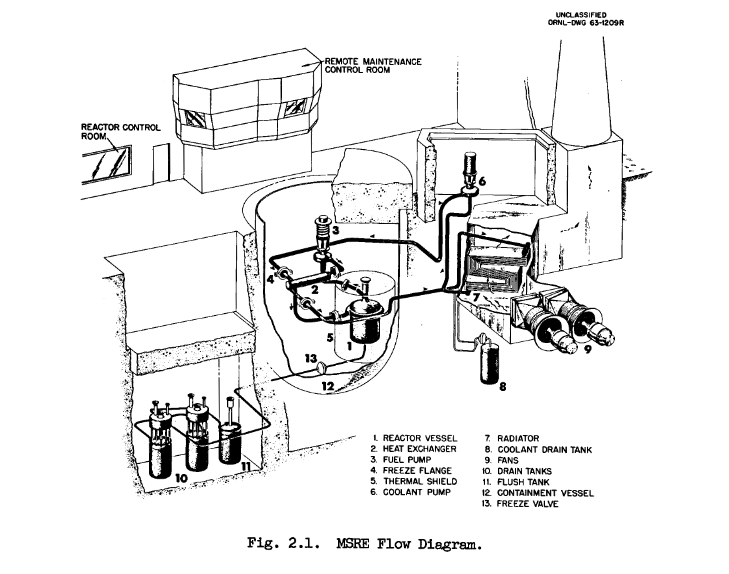
\includegraphics[width=1.0\linewidth]{figures/MSREsource1.png}
  \captionof{figure}{An image of the reactor building setup, from \cite{robertson_msre_1965} directly}
  \label{fig:fig1}
\end{figure}

\begin{figure}[H]
  \centering
  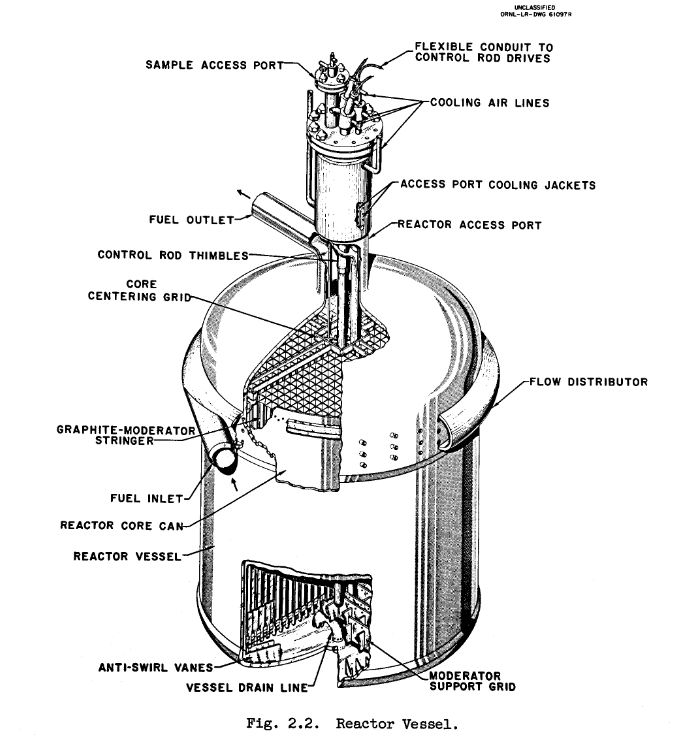
\includegraphics[width=1.0\linewidth]{figures/MSREsource2.png}
  \captionof{figure}{An image of the reactor core, from \cite{robertson_msre_1965} directly}
  \label{fig:fig2}
\end{figure}


\begin{center}
\begin{tabular}{|c|c|}
\hline
Fuel-Moderator Ratio & 22.4-77.6 \\
\hline
Coolant & $LiFBeF_2$ \\
\hline
Moderator & Graphite \\
\hline
Fuel Composition & 2, 3, 4 \\
\hline
\end{tabular}
\end{center}

The fuel processing in the MSRE is relatively straight-forward.  The helium cover gas used in the pump bowl will remove fission product gases.  Beyond the off-gas system, and further fuel processing is done batch-wise, not as part of the fuel loop.  This fuel processing system can:

\begin{itemize}
\item Treat batches of oxygen-contaminated fuel salts with a $H_2F$ gas to remove the oxygen
\item Can perform fluorination on batches of fuel salts.  This will separate the uranium from the salt mixture.  From this point, the salt is either sent to waste, or kept, and a new fuel is added to the batch.  This allows for both "cleaning" the fuel, or changing its composition considerably, in large quantities.
\end{itemize}

\begin{figure}[H]
  \centering
  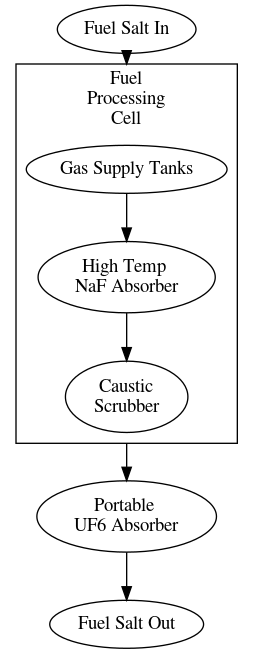
\includegraphics[height=.5\textheight]{figures/msre-proc.png}
  \captionof{figure}{A diagram of the fuel-processing cell of the MSRE}
  \label{fig:figA}
\end{figure}

\begin{figure}[H]
  \centering
  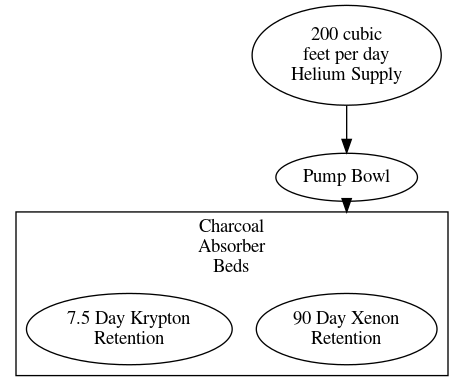
\includegraphics[height=.5\textheight]{figures/msre-offgas.png}
  \captionof{figure}{The off-gas system of the MSRE}
  \label{fig:figB}
\end{figure}

\section{Molten Salt Breeder Reactor (MSBR)}
The MSBR builds on the MSRE, adding a conversion ratio high enough to classify the MSBR as a true breeder reactor.  It features a higher power in its design specifications, at the cost of a low graphite lifetime.  Additionally, it has a lesser fuel vol\% than the MSRE, and two fewer control rods. \cite{bettis_design_1970}, \cite{whatley_engineering_1970}

\begin{center}
\begin{tabular}{|c|c|}
\hline
MWth & 2250 \\
\hline
MWe & 1000 \\
\hline
Spectrum & Thermal \\
\hline
Core Inlet Temperature & 566 C \\
\hline
Core Outlet Temperature & 704 C\\
\hline
Pressure & 0.52 MPa \\
\hline
\end{tabular}
\end{center}

\begin{itemize}
\item Thermal plant efficiency of 44\%
\item Average core power density is approximately 22kW/liter, with a plant factor of 80\%.  This gives:
	\begin{itemize}
	\item A four year graphite lifetime
	\item A fuel yield of 3.3\%
	\item A compounded fuel doubling time of 21 yr
	\end{itemize}
\item Reactor vessel is approximately 22ft in diameter and 20 ft high.
\item Core is 14.3ft in diameter and 13ft high
\item Graphite matrix is a rectangluar grid with 4 control rod slots in the center.
\end{itemize}

\begin{center}
\begin{tabular}{|c|c|}
\hline
Fuel-Moderator Ratio & 13-87 \\
\hline
Moderator & Graphite \\
\hline
Fuel Composition & 5 \\
\hline
Secondary Salt* & $NaBF_4-NaF$ \\
\hline
\end{tabular}
\end{center}

\begin{figure}[H]
  \centering
  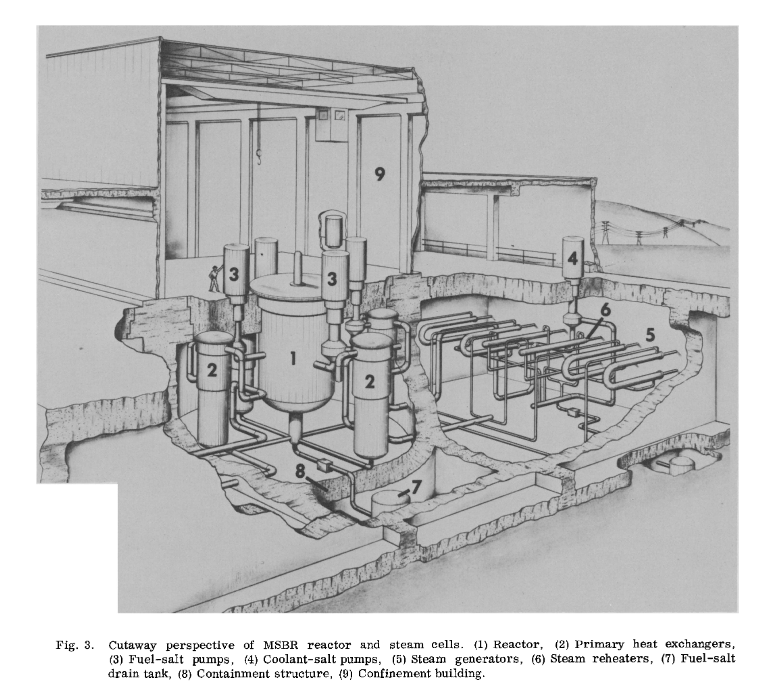
\includegraphics[width=1.0\linewidth]{figures/MSBRsource1.png}
  \captionof{figure}{An image of the reactor and steam systems, from \cite{bettis_design_1970}}
  \label{fig:fig3}
\end{figure}

\begin{figure}[H]
  \centering
  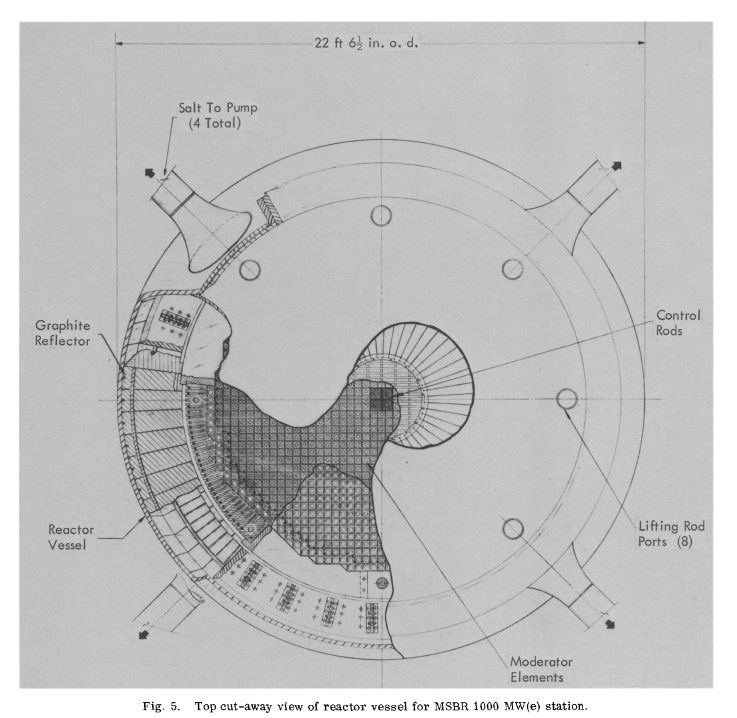
\includegraphics[width=1.0\linewidth]{figures/MSBRsource2.png}
  \captionof{figure}{A bird's eye view of the reactor core, from \cite{bettis_design_1970} }
  \label{fig:fig4}
\end{figure}

The chemical processing is more involved than the MSRE, and includes:
\begin{itemize}
\item An off-gas system to remove gaseous fission products, using helium spargers.
\item A continuous chemical processing loop to:
	\begin{itemize}
	\item Remove fission products
	\item Recover bred ${}^{233}U$
	\item Add more fertile material, as needed.
	\end{itemize}
\end{itemize}

\begin{figure}[H]
  \centering
  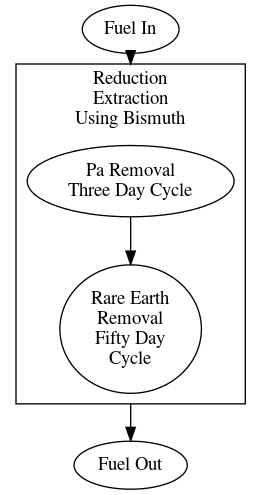
\includegraphics[height=.5\textheight]{figures/msbr-proc.png}
  \captionof{figure}{Material Flow in the MSBR Fuel-Processing Cell}
  \label{fig:figC}
\end{figure}

\begin{figure}[H]
  \centering
  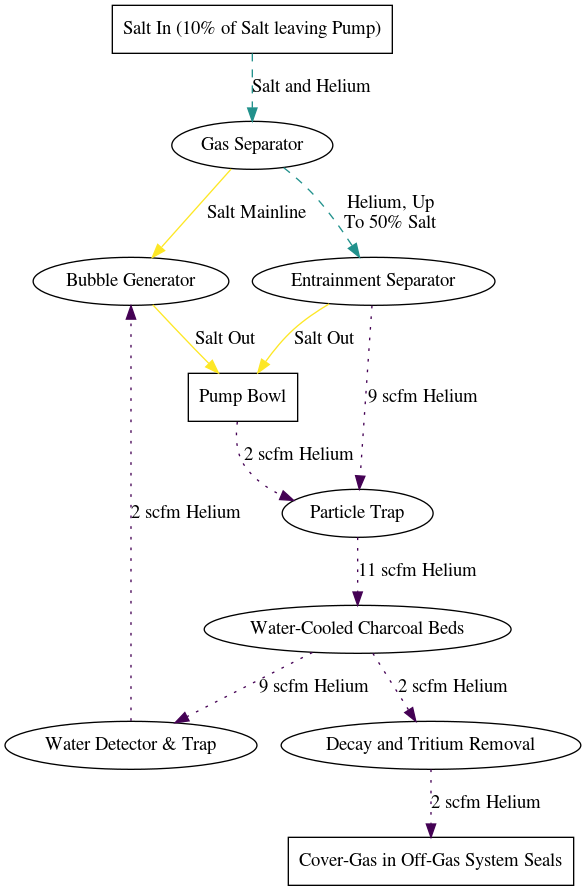
\includegraphics[height=.5\textheight]{figures/msbr-offgas.png}
  \captionof{figure}{The off-gas system in the MSBR}
  \label{fig:figD}
\end{figure}

\section{Molten Salt Demonstration Reactor (MSDR)}
A reactor concept from ORNL, hoping to build on the MSRE and show the commercial capabilities of an MSR.  The intention is to show the feasibility of a breeder MSR, however, the MSDR's conversion ratio isn't high enough to technically be a breeder.  Instead, it is a converter \cite{bettis_design_1972}.  One difference of note between the MSDR and the MSBR is that the  MSDR maintains a low enough power density that the graphite moderator is expected to last 30 years.  This is in stark contrast to the MSBR, which operates at a higher power density, and only anticipates a 4 year graphite lifetime.

\begin{center}
\begin{tabular}{|c|c|}
\hline
MWth & 750 \\
\hline
MWe & 350 \\
\hline
Spectrum & Thermal \\
\hline
Core Inlet Temperature & 566 C\\
\hline
Core Outlet Temperature & 677 C\\
\hline
Pressure & \makecell{Not given explicitly.  Assume\\pressure drop of 0.03 MPa across reflectors.\\Nothing in source to indicate core vessel\\pressure differs significantly from predecessors.} \\
\hline
\end{tabular}
\end{center}

\begin{itemize}
\item Peak power density 114 W/cc
\item Reactor vessel is 26ft tall and 26ft in diameter
\item FLiBe salt, initially using ${}^{235}U$, that uses thorium to breed ${}^{233}U$
\item solid graphite slabs for reflector, arranged in an axial/ radial matrix.  Six slots in the matrix for control rods.
\end{itemize}

\begin{figure}[H]
  \centering
  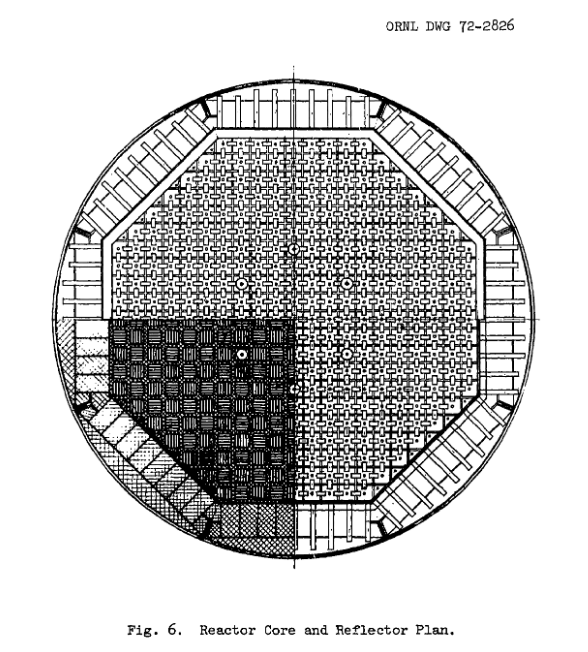
\includegraphics[width=1.0\linewidth]{figures/MSDRsource1.png}
  \captionof{figure}{The layout of the reactor core, from \cite{bettis_design_1972} }
  \label{fig:fig5}
\end{figure}

\begin{figure}[H]
  \centering
  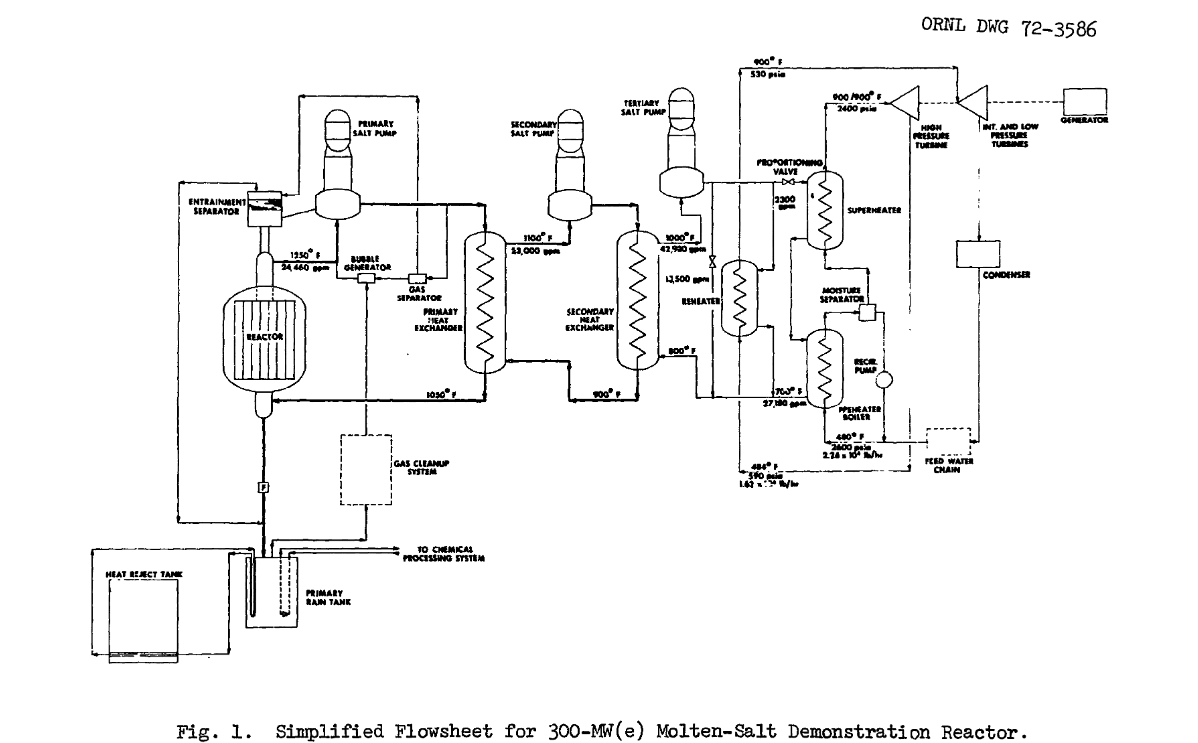
\includegraphics[width=1.0\linewidth]{figures/MSDRsource2.png}
  \captionof{figure}{Layout of the reactor, steam generation, and (most) of the salt processing, from \cite{bettis_design_1972} }
  \label{fig:fig6}
\end{figure}

\begin{center}
\begin{tabular}{|c|c|}
\hline
Fuel-Moderator Ratio & 10-90 \\
\hline
Coolant & $LiFBeF_2$ \\
\hline
Moderator & Graphite \\
\hline
Fuel Composition & 6 \\
\hline
\end{tabular}
\end{center}

The processing used in this reactor is minimal, and is intentionally limited to what was used in the MSRE.  All salt processing is as follows:

\begin{itemize}
\item A Hitec salt loop oxidizes tritium in the fuel salt into tritiated water for removal
	\begin{itemize}
	\item This salt loop goes to the heat exchanger for steam generation
	\end{itemize}
\item Xenon and other fission product gases are removed via an off-gas system
\item Other fission products are not removed from the salt in a short time scale.  Instead, the salt is replaced every 8 years.  Fissile materials are taken from "spent" salt, where possible.
\end{itemize}

\begin{figure}[H]
  \centering
  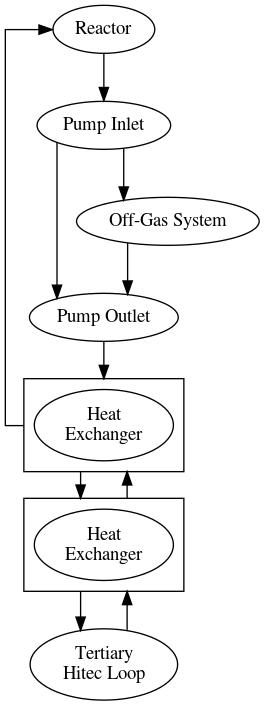
\includegraphics[height=.5\textheight]{figures/msdr-overview.png}
  \captionof{figure}{An overview of the fuel processing in the MSDR design}
  \label{fig:figE}
  
\end{figure}\begin{figure}[H]
  \centering
  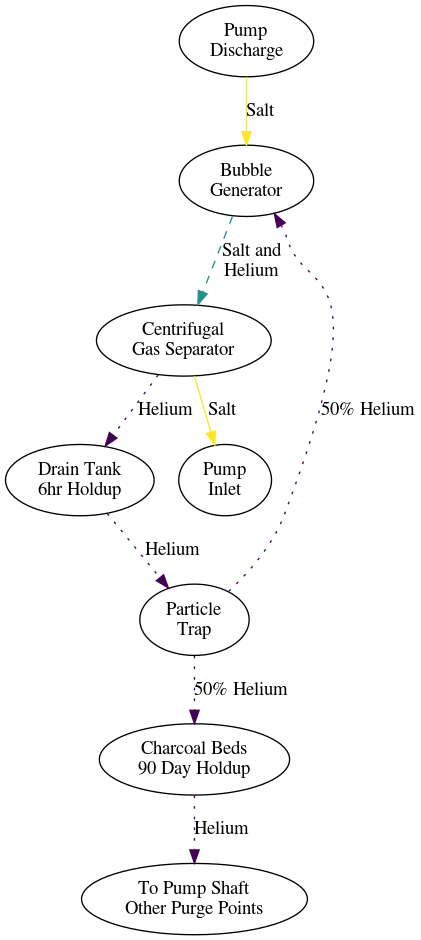
\includegraphics[height=.5\textheight]{figures/msdr-offgas.png}
  \captionof{figure}{The MSDR's off-gas system}
  \label{fig:figF}
\end{figure}

\section{Denatured Molten Salt Reactor (DMSR)}

This reactor is heavily based on the MSBR.  In fact, the design is mostly identical, except the DMSR does not remove fission products during the 30 year lifetime of design.  It does however, include helium sparging and some limited chemical processing to maintain salt quality.  This particular design is prompted by guidance given in 1976 by what is now the DOE, along with reports that concluded a breeder reactor without denatured fuel would not be able to be deployed worldwide, due to insufficient proliferation resistance. \cite{engel_conceptual_1980}

The basic core parameters are as follows:

\begin{center}
\begin{tabular}{|c|c|}
\hline
MWth & 2250 \\
\hline
MWe & 1000 \\
\hline
Spectrum & Thermal \\
\hline
Core Inlet Temperature & 566 C \\
\hline
Core Outlet Temperature & 704 C\\
\hline
Pressure & Not given \\
\hline
\end{tabular}
\end{center}

\begin{itemize}
\item Low power density to give the graphite moderator a 30 year lifetime.
	\begin{itemize}
	\item Low power density also reduces neutron capture in ${}^{233}Pa$, to bolster nonproliferation
	\end{itemize}
\item Uses 20\% enriched ${}^{235}U$ to reach initial criticality.
\item Like the MSBR, uses $LiF - BeF_2 - ThF_4 - UF_4$ salt (with the above change in fissile isotope)
\item This reactor vessel is 10m in both height diameter, with the following core specifications:
	\begin{itemize}
	\item The core is 8.3m in height and diameter.
		\begin{itemize}
		\item The outer 95\% of the core volume, core B, has a salt volume of 12.94\%
		\item The inner 5\% of the core, core A, has a salt volume of 20\%
		\end{itemize}
	\end{itemize}
\item Table 9 and Table 10 in \cite{engel_conceptual_1980} give isotope concentrations and neutron utilization, as calculated for a few points in the reactor lifetime.
\end{itemize}

\begin{figure}[H]
  \centering
  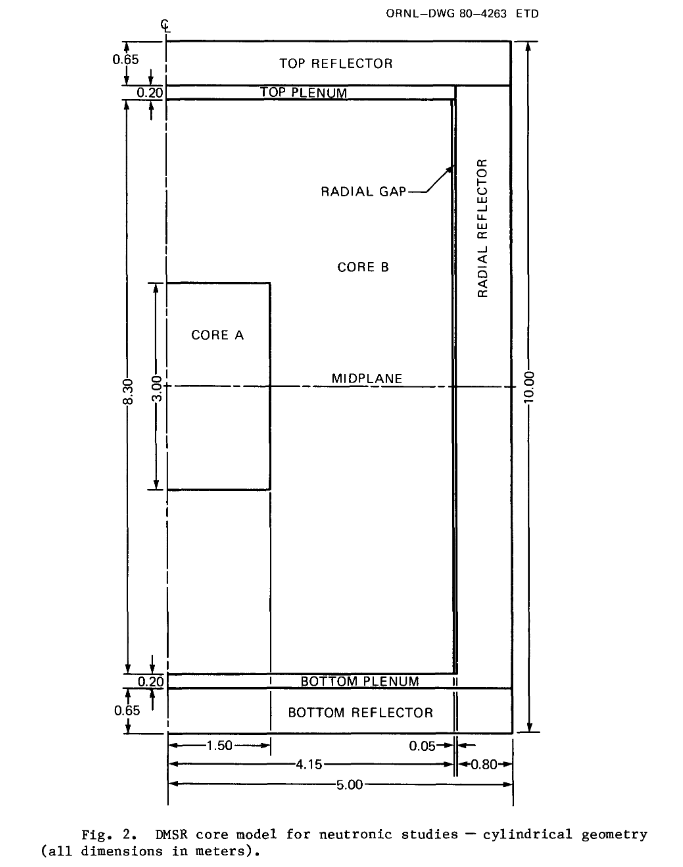
\includegraphics[width=1.0\linewidth]{figures/DMSRsource1.png}
  \captionof{figure}{A cut-away view of the core, from \cite{engel_conceptual_1980} }
  \label{fig:fig7}
\end{figure}

\begin{center}
\begin{tabular}{|c|c|}
\hline
Fuel-Moderator Ratio: Inner Core & 20-80 \\
\hline
Fuel-Moderator Ratio: Outer Core & 12.94-87.06  \\
\hline
Coolant & $LiFBeF_2$ \\
\hline
Moderator & Graphite \\
\hline
Fuel Composition & 7 \\
\hline
\end{tabular}
\end{center}

As stated previously, the reprocessing in this design is purposefully limited in order to improve the fuel cycle's proliferation resistance.  The desig includes an off-gas system, which will remove gaseous fission products.  Aside from this, however, the only other treatment the fuel recieves is what is necessary to keep oxygen-contamination to a minimum, and to maintain the proper levels of fissile isotopes within the fuel.  The DMSR does not include the liquid-metal reduction-extraction commonly seen in previous designs, and does not, at any point, separate protactinium.  The design assumes noble metals will leave the fuel by plating out on the piping.

\begin{figure}[H]
  \centering
  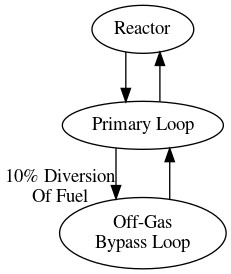
\includegraphics[height=.5\textheight]{figures/dmsr-proc.png}
  \captionof{figure}{The diversion of salt to the off-gas system}
  \label{fig:figG}
\end{figure}

\section{Integral Molten Salt Reactor (IMSR)}

The IMSR400 is a small modular reactor (SMR) patented by Terrestrial Energy Inc.  The "core-unit" consists of the reactor vessel, and integrated pumps and heat exchangers.  The core-unit has a lifetime of 7 years, but is made to be easily replaced, giving the designed plant an expected lifetime of 30 years.  Some specifics of this reactor, such as the fuel-coolant mixture, is proprietary, and explicit detail is not given.  What information is publicly available is as follows \cite{leblanc_18_2017}:

\begin{center}
\begin{tabular}{|c|c|}
\hline
MWth & 400 \\
\hline
MWe & 188 \\
\hline
Spectrum & Thermal \\
\hline
Core Inlet Temperature & 647 C \\
\hline
Core Outlet Temperature & 685 C\\
\hline
Pressure & 0.4 MPa \\
\hline
\end{tabular}
\end{center}

\begin{itemize}
\item Average core power density of 11-15 $\frac{MW}{m^{3}}$
\item Core is 4m in height, and 3.4m in diameter.
\item The length of each fuel cycle is 84 months, i.e., the 7-year lifetime of the core-unit
\item The moderator is graphite, the shutdown rods are made of gadolinium oxide, and it does not have control rods
\item At the time of discharge, the average burnup is 26-29 MWd/kg
\item The salt mixture is a blend of fluoride salts, including sodium fluoride, berylium fluoride, and lithium fluoride.  At startup, the fuel has an enrichment of 2-3\%, and an enrichment of 5-19\% when used fissile material is replaced
\end{itemize}

\begin{figure}[H]
  \centering
  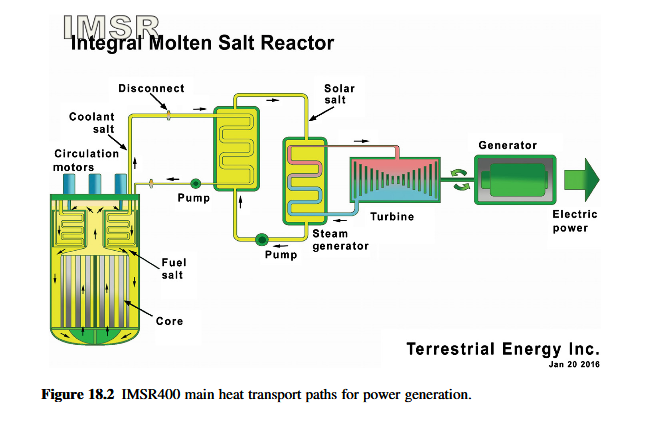
\includegraphics[width=1.0\linewidth]{figures/IMSRsource1.png}
  \captionof{figure}{A simplified view of the core-unit, and its attachment to the power generation loops, from \cite{leblanc_18_2017} }
  \label{fig:fig8}
\end{figure}

\begin{figure}[H]
  \centering
  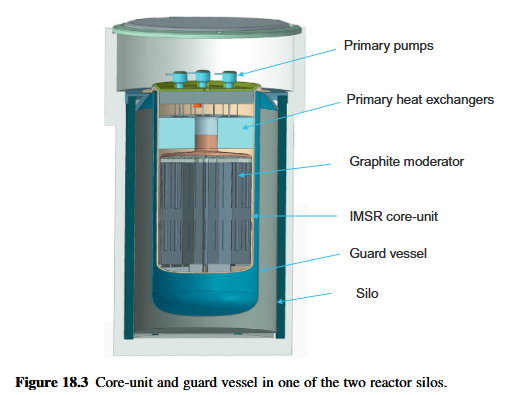
\includegraphics[width=1.0\linewidth]{figures/IMSRsource2.png}
  \captionof{figure}{The core, from \cite{leblanc_18_2017} }
  \label{fig:fig9}
\end{figure}

\begin{center}
\begin{tabular}{|c|c|}
\hline
Fuel-Moderator Ratio & Not Given \\
\hline
Coolant & "Fluoride Salt" \\
\hline
Moderator & Graphite \\
\hline
Fuel Composition & "Fluoride Fuel Salt" \\
\hline
\end{tabular}
\end{center}

\section{Molten Salt Fast Reactor (MSFR)}
Of the reactors given in this review, this is the only one using the fast spectrum (certainly, other fast-MSRs exist, but may not necessarily be interesting from a fuel-processing stand point).  Because such a reactor does not use a moderator, it circumvents some of the material contraints associated with degradation of the graphite moderator.  It also has a much higher breeding ratio.  This report uses a conceptual reference reactor with these characteristics \cite{rouch_preliminary_2014}: 

\begin{center}
\begin{tabular}{|c|c|}
\hline
MWth & 3000 \\
\hline
MWe & 1500 \\
\hline
Spectrum & Fast \\
\hline
Core Inlet Temperature & 625 C \\
\hline
Core Outlet Temperature & 730 C \\
\hline
Pressure & Not Given \\
\hline
\end{tabular}
\end{center}

\begin{itemize}
\item Three loops: the fuel, intermediate, and power conversion loops
\item Within the fuel circuit, there is a total salt volume of 18 cubic meters
	\begin{itemize}
	\item The fuel salt is lithium fluoride and actinide fluoride, with the mol\% of the actinide fluorides is assumed to be a fixed 22.5 mol\%
	\end{itemize}
\item Within the core, there is a fertile isotope blanket region, composed of a $LiF - ThF_4$ blend that has a concentration of $ThF_4$ of 22.5 mol\%
\item The blanket serves as the radial reflectors, to protect the reactor vessel.  On the top and bottom, there are reflectors made of nickel-based alloys.  This particular report also assumes this alloy will absorb 99\% of incoming neutrons.
\item The design initially used a very simple cylindrical geometry for the core, but by the time the report was written, the study moved on to more realistic, and complicated, geometries.
	\begin{itemize}
	\item The first geometry is referred to as Geometry I.  The radial core walls are curved, along with the top reflector.  The bottom reflector is flat
	\item The second Geometry, Geometry II, features symmetrically curved walls within the core.  Both this and Geometry I are given in \ref{fig10} below.
	\end{itemize}
\item Helium sparging is assumed, but because its impact and the thermal-hydraulic properties was deemed neglible, it is neglected in calculations
\end{itemize} 

\begin{figure}[H]
  \centering
  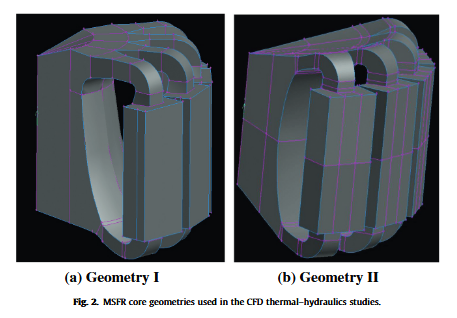
\includegraphics[width=1.0\linewidth]{figures/MSFRsource1.png}
  \captionof{figure}{Geometries I and II, from \cite{rouch_preliminary_2014}}
  \label{fig:fig10}
\end{figure}


In a separate report, \cite{doligez_coupled_2014} , a reactor with the same nominal power, and actinide mol\% is studied.   While \cite{rouch_preliminary_2014} is focused on the thermal-hydraulic facets of an MSFR, \cite{doligez_coupled_2014} provides more in-depth information about the sort of fuel salt composition used in its reference model, and includes information on the reprocessing within the reference MSFR.

\begin{itemize}
\item This report gives the fissile salt explicitly: $LiF - ThF_4 - {}^{233}UF_4$ in with mol\% concentrations of $77.5\% - 20\% - 2.5\%$
\item The fertile blanket is 50 cm thick
\item The initial blanket salt is identical to the above report - $LiF - ThF_4$ in mol\% concentrations of $77.5\% - 22.5\%$

\end{itemize}
\begin{center}
\begin{tabular}{|c|c|}
\hline
Fuel-Moderator Ratio & 100-0 \\
\hline
Coolant & \makecell{As fuel salt, without\\fuel isotopes.} \\
\hline
Moderator & No moderator \\
\hline
Fuel Composition & 8, 9 \\
\hline
\end{tabular}
\end{center}

\begin{figure}[H]
  \centering
  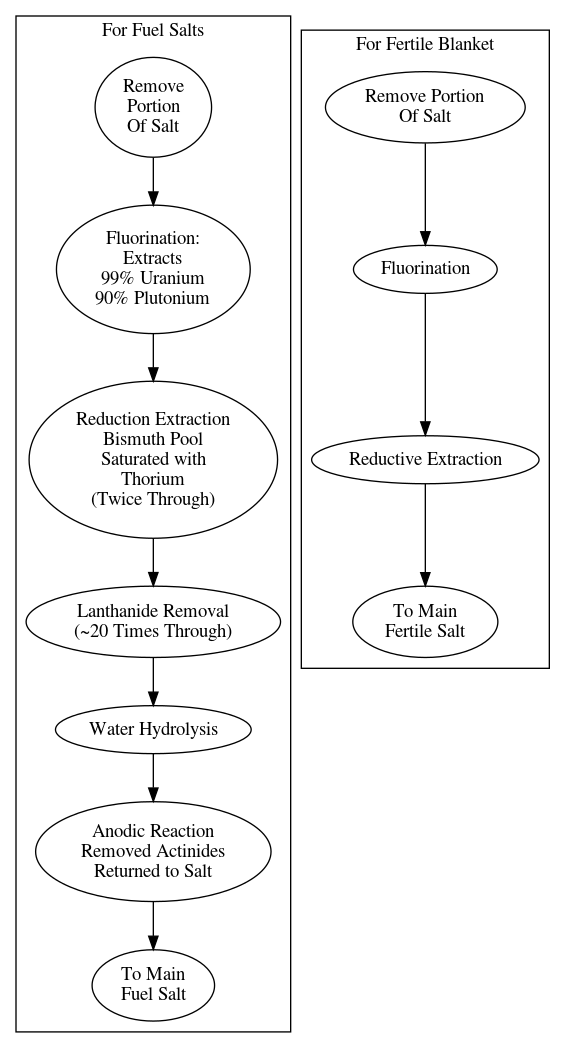
\includegraphics[height=.5\textheight]{figures/msfr-proc.png}
  \captionof{figure}{Fuel processing in the MSFR}
  \label{fig:figH}
\end{figure}

\begin{figure}[H]
  \centering
  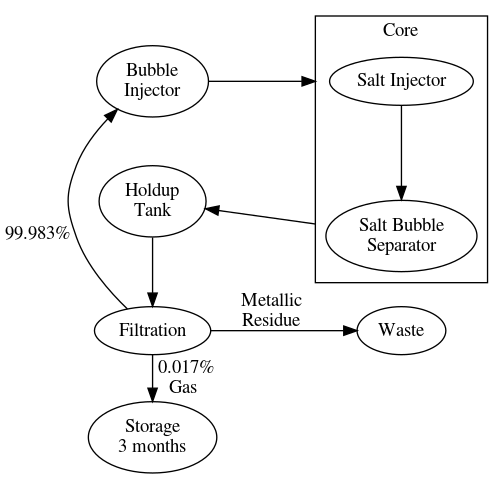
\includegraphics[height=.5\textheight]{figures/msfr-offgas.png}
  \captionof{figure}{The off-gas system of the MSFR}
  \label{fig:figI}
\end{figure}

\section{Transatomic}

The Transatomic reactor has two important differences from other thermal-spectrum MSRs in this review.  It changes the fuel salt mixture, and forgoes a graphite moderator for something with a better lifespan under the conditions of the reactor \cite{robertson_assessment_2017} \cite{transatomic_power_corporation_neutronics_2016} \cite{transatomic_power_corporation_technical_2016}.

\begin{center}
\begin{tabular}{|c|c|}
\hline
MWth & 1250 \\
\hline
MWe & 520 \\
\hline
Spectrum & Thermal \\
\hline
Core Inlet Temperature & Not Given \\
\hline
Core Outlet Temperature & 650 C\\
\hline
Pressure & "Near-Atmospheric" \\
\hline
\end{tabular}
\end{center}

\begin{itemize}
\item The fuel salt is a $LiF - UF_4$ mixture, with a uranium concentration of 27.5\%
\item Unlike the other MSR designs reviewed, the Transatomic reactor uses a zirconium hydride moderator with corrosion resistant cladding
	\begin{itemize}
	\item Table 1 of \cite{robertson_assessment_2017} gives dimensional parameters for the moderator rods in the core
	\end{itemize}
\item Transtomic has proposed three fueling scenarios, but only the first has been the focus of ORNL studies:
	\begin{enumerate}
	\item 5\% start-up enrichment, followed by a 5\% online feed
	\item 5\% start-up enrichment, followed by an online feed of spent fuel from light water reactors
	\item 10\% start-up enrichment, followed by an online feed of 19.9\%
	\end{enumerate}
\item Burnup can be as high as 200 MWd/MTU, with the intention of limiting waste products
	\begin{itemize}
	\item After analysis of core models, with simulation of the chemical processing included with use of ChemTriton, the report concludes that after 15 years of operation, the reactor has bred enough plutonium to reach a burnup of 91.9 GWd/MTU by year 29.1 of operation
	\end{itemize}
\end{itemize}

\begin{center}
\begin{tabular}{|c|c|}
\hline
Fuel-Moderator Ratio & Not Given \\
\hline
Coolant & $FLiNaK$ \\
\hline
Moderator & Zirconium Hydride \\
\hline
Fuel Composition & 10 \\
\hline
\end{tabular}
\end{center}


\bibliographystyle{plain}
\bibliography{2019-richter-msr-litrev.bib}
\end{document}
